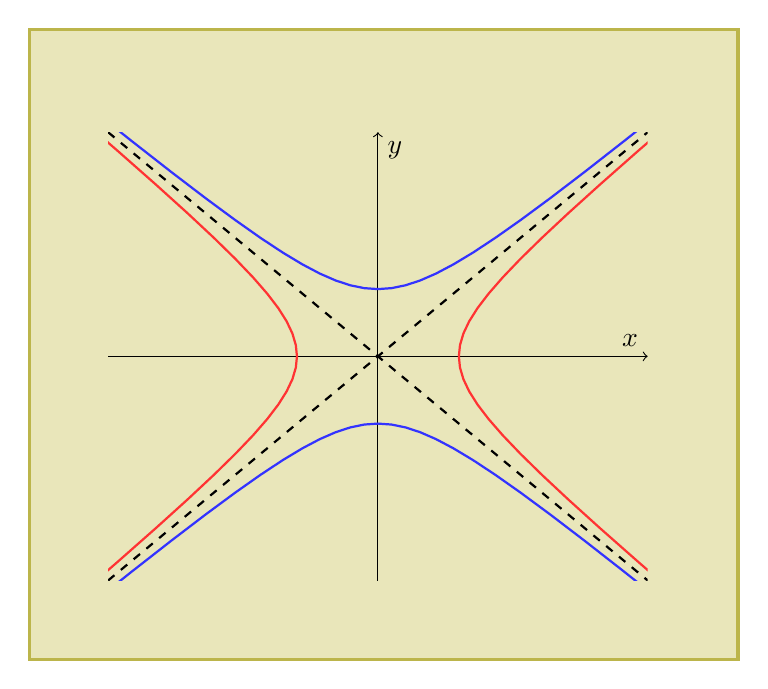
\begin{tikzpicture}
  \draw[draw = olive!60, fill = olive!20, very thick]
    (-1, -1) rectangle (8, 7);

  \begin{axis}[
    xmin = -5,
    xmax = 5,
    ymin = -5,
    ymax = 5,
    axis x line = middle,
    axis y line = middle,
    xlabel = {\(x\)},
    ylabel = {\(y\)},
    axis line style = {->},
    ticks = none,
  ]
    \addplot[thick, red!80, domain = -2 : 2]
      ({ 1.5 * cosh(x) }, { 1.5 * sinh(x) });
    \addplot[thick, red!80, domain = -2 : 2]
      ({ -1.5 *  cosh(x) }, { 1.5 * sinh(x) });
    \addplot[thick, blue!80, domain = -2 : 2]
      ({ 1.5 * sinh(x) }, { 1.5 * cosh(x) });
    \addplot[thick, blue!80, domain = -2 : 2]
      ({ 1.5 * sinh(x) }, { -1.5 * cosh(x) });

    \addplot[dashed, thick] expression {x};
    \addplot[dashed, thick] expression {-x};
  \end{axis}
\end{tikzpicture}